\section{Iteración II}
\subsection{Resumen}
En esta iteración se modelo un mueble y se implementó para visualizarse en la aplicación.
\subsection{Desarrollo}
Ya entendido el funcionamiento de ARcore y como agregar nuevos modelos, en esta iteración se modelo el primer mueble, al igual que en la iteración pasada se obtuvieron dos tipos de archivos y se renderizaron para mostrarse en la aplicación.
\begin{figure}[H]
	\centering
	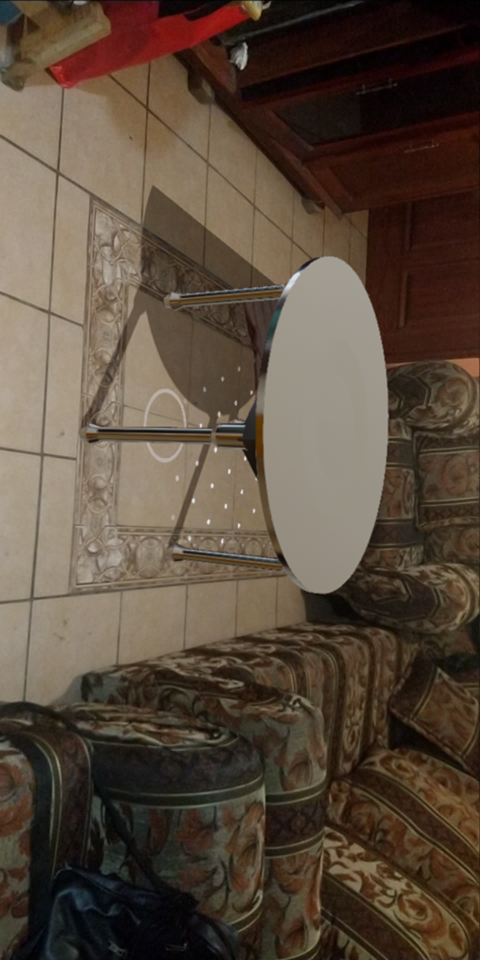
\includegraphics[width=8cm,height=14cm,angle=90]{imagenes/iteraciones/AR3.png}
	\caption{Mueble modelado en 3D}
	\label{fig:analogo}
\end{figure} 
